The development board is from Renesas\footnote{A joint venture of NEC, Mitsubishi and Hitachi}. 

The ZMD28-BRD is taken from the ZigBee Demonstration Kit with the part number RZB-CC16C-ZDK.
Main features include a M16C TinyMCU, a photo and temperature sensor, LEDs for custom use, a two-lined LCD and a RS232
connection for programming and possible host machines. The board uses ZigBee as means of wireless communication.
\cite{RenesasZDK}

\begin{figure}[H]
   \centering
   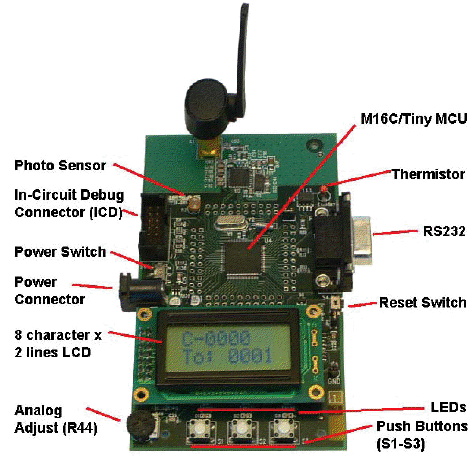
\includegraphics[width=0.6\textwidth]{pic/wsn.png}%
   \caption{2.4GHz ZDK Board(Source: Renesas Documentation)}
   \label{wsnpic}%
\end{figure}

It is capable to serve as route and coordinator in a ZigBee-Network. On default the modes are selectable by
pressing the first or second button on starting up a vanilla board. The behaviour is customizable with 
software programming. Basically a rough start is available through the included RTOS and the ZigBee stack which
is included in the ZDK.

\section{ZigBee}

BLABLA
